\documentclass[border=6pt]{standalone}
\usepackage{amsmath,amssymb}
\usepackage{tikz}
\usetikzlibrary{arrows.meta,calc,decorations.pathreplacing,patterns,shapes.geometric,positioning,shadings,plotmarks}

\begin{document}
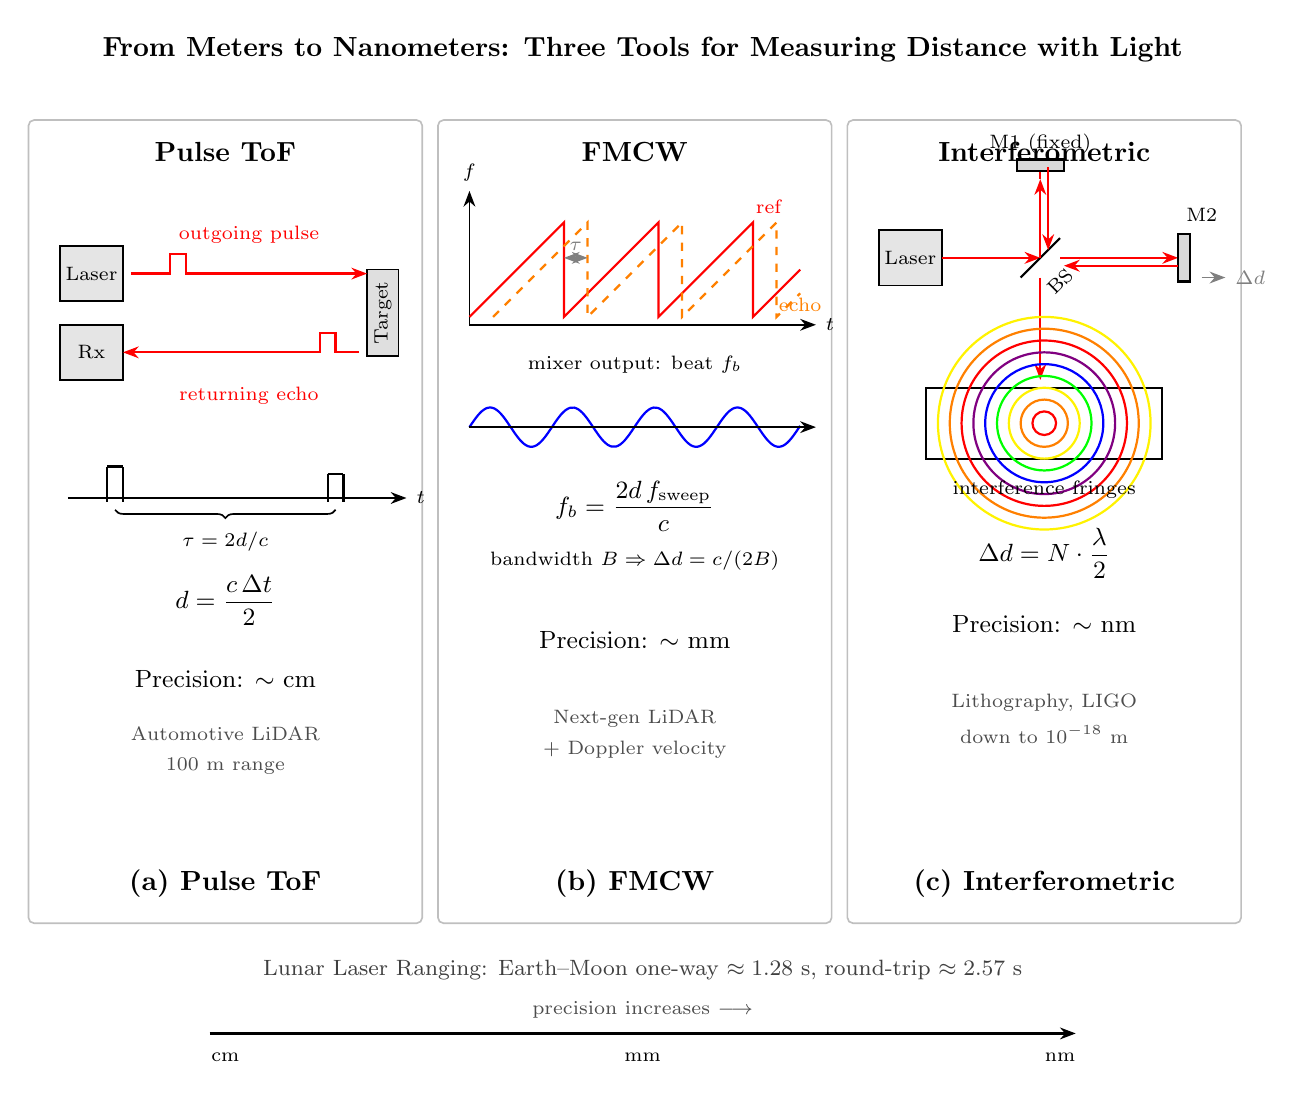
\begin{tikzpicture}[
    >={Stealth[length=2mm,width=1.5mm]},
    line width=0.6pt,
    font=\small
]

% ============ TITLE ============
\node[font=\bfseries] at (7.5,7.5) {From Meters to Nanometers: Three Tools for Measuring Distance with Light};

% ============ LEFT COLUMN: PULSE ToF ============
\begin{scope}[xshift=0cm]
  % Column frame
  \draw[rounded corners=2pt, gray!50] (-0.3,-3.6) rectangle (4.7,6.6);
  \node[font=\bfseries] at (2.2,6.2) {Pulse ToF};

  % Laser transmitter
  \draw[fill=black!10] (0.1,4.3) rectangle (0.9,5.0);
  \node[font=\scriptsize] at (0.5,4.65) {Laser};
  % Receiver
  \draw[fill=black!10] (0.1,3.3) rectangle (0.9,4.0);
  \node[font=\scriptsize] at (0.5,3.65) {Rx};

  % Target
  \draw[fill=gray!25] (4.0,3.6) rectangle (4.4,4.7);
  \node[font=\scriptsize, rotate=90] at (4.2,4.15) {Target};

  % Outgoing pulse (square wave red)
  \draw[red,thick] (1.0,4.65) -- (1.5,4.65) -- (1.5,4.9) -- (1.7,4.9) -- (1.7,4.65) -- (3.9,4.65);
  \draw[red,->] (3.9,4.65) -- (4.0,4.65);
  \node[font=\scriptsize,red] at (2.5,5.15) {outgoing pulse};

  % Returning pulse
  \draw[red,thick] (3.9,3.65) -- (3.6,3.65) -- (3.6,3.9) -- (3.4,3.9) -- (3.4,3.65) -- (1.0,3.65);
  \draw[red,->] (1.0,3.65) -- (0.9,3.65);
  \node[font=\scriptsize,red] at (2.5,3.1) {returning echo};

  % Time axis
  \draw[->] (0.2,1.8) -- (4.5,1.8) node[right,font=\scriptsize] {$t$};
  \draw[thick] (0.7,1.75) -- (0.7,2.2);
  \draw[thick] (0.9,1.75) -- (0.9,2.2);
  \draw[thick] (0.7,2.2) -- (0.9,2.2);
  \draw[thick] (3.5,1.75) -- (3.5,2.1);
  \draw[thick] (3.7,1.75) -- (3.7,2.1);
  \draw[thick] (3.5,2.1) -- (3.7,2.1);
  % Tau bracket
  \draw[decorate,decoration={brace,amplitude=3pt,mirror}] (0.8,1.65) -- (3.6,1.65);
  \node[font=\scriptsize] at (2.2,1.25) {$\tau = 2d/c$};

  % Formula
  \node at (2.2,0.5) {$d = \dfrac{c\,\Delta t}{2}$};

  % Precision
  \node[font=\small] at (2.2,-0.5) {Precision: $\sim$ cm};

  % Application
  \node[font=\scriptsize,gray!60!black] at (2.2,-1.2) {Automotive LiDAR};
  \node[font=\scriptsize,gray!60!black] at (2.2,-1.6) {100 m range};

  % Label
  \node[font=\bfseries] at (2.2,-3.1) {(a) Pulse ToF};
\end{scope}

% ============ MIDDLE COLUMN: FMCW ============
\begin{scope}[xshift=5.2cm]
  \draw[rounded corners=2pt, gray!50] (-0.3,-3.6) rectangle (4.7,6.6);
  \node[font=\bfseries] at (2.2,6.2) {FMCW};

  % Frequency-time plot
  \draw[->] (0.1,4.0) -- (0.1,5.7) node[above,font=\scriptsize] {$f$};
  \draw[->] (0.1,4.0) -- (4.5,4.0) node[right,font=\scriptsize] {$t$};

  % Reference sawtooth (red)
  \draw[red,thick] (0.1,4.1) -- (1.3,5.3) -- (1.3,4.1) -- (2.5,5.3) -- (2.5,4.1) -- (3.7,5.3) -- (3.7,4.1) -- (4.3,4.7);
  % Echo sawtooth shifted by tau (orange)
  \draw[orange,thick,dashed] (0.4,4.1) -- (1.6,5.3) -- (1.6,4.1) -- (2.8,5.3) -- (2.8,4.1) -- (4.0,5.3) -- (4.0,4.1) -- (4.3,4.4);

  \node[font=\scriptsize,red] at (3.9,5.5) {ref};
  \node[font=\scriptsize,orange] at (4.3,4.25) {echo};

  % Tau shift indicator
  \draw[<->,gray] (1.3,4.85) -- (1.6,4.85);
  \node[font=\scriptsize,gray] at (1.45,5.0) {$\tau$};

  % Beat frequency sinusoid (blue) below
  \node[font=\scriptsize] at (2.2,3.5) {mixer output: beat $f_b$};
  \draw[blue,thick,domain=0.1:4.3,samples=80,smooth] plot (\x,{2.7+0.25*sin(deg((\x-0.1)*6))});
  \draw[->] (0.1,2.7) -- (4.5,2.7);

  % Formula
  \node at (2.2,1.7) {$f_b = \dfrac{2 d\, f_{\text{sweep}}}{c}$};
  \node[font=\scriptsize] at (2.2,1.0) {bandwidth $B \Rightarrow \Delta d = c/(2B)$};

  % Precision
  \node[font=\small] at (2.2,0.0) {Precision: $\sim$ mm};

  % Application
  \node[font=\scriptsize,gray!60!black] at (2.2,-1.0) {Next-gen LiDAR};
  \node[font=\scriptsize,gray!60!black] at (2.2,-1.4) {+ Doppler velocity};

  \node[font=\bfseries] at (2.2,-3.1) {(b) FMCW};
\end{scope}

% ============ RIGHT COLUMN: INTERFEROMETRIC ============
\begin{scope}[xshift=10.4cm]
  \draw[rounded corners=2pt, gray!50] (-0.3,-3.6) rectangle (4.7,6.6);
  \node[font=\bfseries] at (2.2,6.2) {Interferometric};

  % Laser source
  \draw[fill=black!10] (0.1,4.5) rectangle (0.9,5.2);
  \node[font=\scriptsize] at (0.5,4.85) {Laser};

  % Beam from laser to beam splitter
  \draw[red,thick,->] (0.9,4.85) -- (2.15,4.85);

  % Beam splitter (diagonal line)
  \draw[thick] (1.9,4.6) -- (2.4,5.1);
  \node[font=\scriptsize,rotate=45] at (2.4,4.55) {BS};

  % Reference arm (fixed mirror up)
  \draw[red,thick,->] (2.15,4.85) -- (2.15,5.85);
  \draw[red,thick] (2.15,5.85) -- (2.15,5.95);
  \draw[thick,fill=gray!30] (1.85,5.95) rectangle (2.45,6.1);
  \node[font=\scriptsize] at (2.15,6.3) {M1 (fixed)};

  % Reflected back
  \draw[red,thick,->] (2.25,6.0) -- (2.25,4.95);

  % Measurement arm (movable mirror right)
  \draw[red,thick,->] (2.4,4.85) -- (3.9,4.85);
  \draw[thick,fill=gray!30] (3.9,4.55) rectangle (4.05,5.15);
  \node[font=\scriptsize] at (4.2,5.4) {M2};
  \draw[->,gray] (4.2,4.6) -- (4.5,4.6) node[right,font=\scriptsize] {$\Delta d$};

  % Back toward BS
  \draw[red,thick,->] (3.9,4.75) -- (2.45,4.75);

  % Output beam down to screen
  \draw[red,thick,->] (2.15,4.6) -- (2.15,3.3);

  % Fringe screen (concentric rings simulated with color bands)
  \draw[thick] (0.7,2.3) rectangle (3.7,3.2);
  \foreach \r/\c in {0.15/red,0.3/orange,0.45/yellow,0.6/green,0.75/blue,0.9/violet,1.05/red,1.2/orange,1.35/yellow} {
    \draw[\c,thick] (2.2,2.75) circle (\r);
  }
  \node[font=\scriptsize] at (2.2,1.9) {interference fringes};

  % Formula
  \node at (2.2,1.1) {$\Delta d = N \cdot \dfrac{\lambda}{2}$};

  % Precision
  \node[font=\small] at (2.2,0.2) {Precision: $\sim$ nm};

  % Application
  \node[font=\scriptsize,gray!60!black] at (2.2,-0.8) {Lithography, LIGO};
  \node[font=\scriptsize,gray!60!black] at (2.2,-1.2) {down to $10^{-18}$ m};

  \node[font=\bfseries] at (2.2,-3.1) {(c) Interferometric};
\end{scope}

% ============ BOTTOM NOTE ============
\node[font=\footnotesize,gray!50!black] at (7.5,-4.2) {Lunar Laser Ranging: Earth--Moon one-way $\approx 1.28$ s, round-trip $\approx 2.57$ s};

% Scale bar below showing precision progression
\draw[thick,->] (2.0,-5.0) -- (13.0,-5.0);
\node[font=\scriptsize] at (2.2,-5.3) {cm};
\node[font=\scriptsize] at (7.5,-5.3) {mm};
\node[font=\scriptsize] at (12.8,-5.3) {nm};
\node[font=\scriptsize,gray!60!black] at (7.5,-4.7) {precision increases $\longrightarrow$};

\end{tikzpicture}
\end{document}
